\clearpage
\section{What the models contain: the detail}\label{app:interp-detail}

This appendix holds the detail behind \cref{sec:interp}: the identity checks of the analyses and DFG's small-$n$ choices (\cref{app:interp-fits}), the models family by family (\cref{app:interp-families}), the spurious terms (\cref{app:interp-spur}), the comparison with v3's DFG member (\cref{app:interp-v3}), false admissions (\cref{app:interp-calib}), h5s1's refits (\cref{app:interp-h5s1}), when structure appears (\cref{app:interp-when}) and the order of acquisition (\cref{app:interp-order}). Most of it is seed 0, from \repo{study/part11/interp/ATLAS.md}, \repo{study/part11/interp/calib/CALIB.md}, \repo{study/part11/interp/theory/THEORY.md}, \repo{study/part11/interp/order/ORDER.md} and \repo{study/part11/interp/ablations/ABLATIONS.md}, each with its verification.

% ------------------------------------------------------------------------------------------------------------------
\subsection{The analyses' fits, and DFG's choices at small \texorpdfstring{$n$}{n}}\label{app:interp-fits}

\paragraph{The wrapper} \status{Numerical}. The analyses refit DFG through one wrapper (\repo{study/part11/interp/dfg_hooks.py}). It loads the frozen file (md5 checked), builds the training rows, the fit's random stream and the column permutation exactly as the evaluation does, and records every call of DFG's fit routine without changing it: at $n\le512$ the $2F$ fold fits of the cross-validation, then the final fit on all $n$ rows, whose model predicts. 517 seed-0 cells (47 targets of all 11 suites, every grid $n$) reproduce the test error and the FLOP count of the result files bit for bit, as do 66 cells of the runs at $d=15$, 60 and 120 (\repo{study/part11/interp/tables/identity.md}). The result files store no models, so the identity is of errors and FLOP counts, a strong fingerprint of the same code path. The other analyses pass the same check:
\begin{itemize}
\item \emph{The atlas}: 517 cells at $d=30$ (47 targets of all 11 suites, every $n$, seed 0) and 66 cells at $d=15$, 60 and 120, equal in test error and FLOP count (\repo{study/part11/interp/tables/identity.md}).
\item \emph{The order analysis}: 363 fits (11 \code{designed} targets, every $n$, seeds 0--2), equal in both; the residual rebuilt from the recorded weights matches DFG's own round log in all of them (\repo{study/part11/interp/order/ORDER.md}).
\item \emph{The theory checks}: 330 new seed-0 cells of \code{designed} and \code{random}, equal in both, and the 110 fits on null labels, whose round-0 decisions an independent replica reproduces in all 110 (\repo{study/part11/interp/theory/THEORY.md}).
\item \emph{The false-admission and compute analysis} runs an instrumented copy of the frozen file with 64 inserted lines that only read. Its verifier rebuilt the copy byte for byte and found that removing the inserted statements leaves a syntax tree identical to the frozen file's. Every fit checked against the frozen module or the result files is equal (88 on noise, 451 on the designed and random targets, 35 profiled cells), and the unchecked fits are equal by that construction (\repo{study/part11/interp/calib/VERIFY_CALIB.md}).
\item \emph{This paper's check} of h5s1 (\cref{sec:interp-fail}): 6 refits, equal in test error (\repo{paper_dfg/check_h5s1.json}).
\end{itemize}
\emph{The ablation analysis}: All 38 refits of the analysis, and the 42 made when its verification was applied, reproduce their run's result file exactly in test error and FLOP count (\repo{study/part11/interp/ablations/results/refits.json}, \texttt{refits\_verif.json}). In four cells the same fit through the evaluation's own loader of the frozen file gives the same model, term by term (\repo{study/part11/interp/ablations/results/refit_crosscheck.json}).

\paragraph{Terms, term s.d.\ and categories, in full.} A model is read as terms in the original input coordinates, with the column permutation undone: the constant, each character $\chi_S$, each spectral feature, each sum block with all its level indicators as one term, and the kernel background. A term's \emph{s.d.}\ is the standard deviation of its contribution to the model's output over the 4096 test inputs (an absolute standard deviation, not a fraction of the output's); a group's \emph{share} is that of its summed contribution, as a fraction of the output's. A term is a \emph{target term} (T) if it is a character in the target's Fourier support or in one of its compact representations, or a block with a true class's input set and signs. It is \emph{relevant} (R) if it reads only relevant inputs but is not a target term, and \emph{spurious} (S) if it reads an irrelevant one. S-lin marks the irrelevant degree-1 characters that entered with the linear block, which adds every input not yet in the model.

\paragraph{The target's own representations.} For each target the atlas writes down the compact representations it has in DFG's dictionary (\repo{study/part11/interp/atlas_truth.py}). They are the sign of a few characters (parities, staircases, majorities of parities, halfspaces, DNFs, CNFs, decision lists), the exact Fourier expansion (multiplexers, random and read-once formulas), and sum blocks on the target's signed-symmetry classes, additive, modulated, weighted or as a product. Character representations are verified on all $2^k$ assignments of the $k$ relevant inputs. Block representations are checked only as ``$f$ is a function of the block statistics''; their accept sets are not checked.

\paragraph{Complete, exact, and what the features can express.} A representation is \emph{complete} in a model when all its characters are present, or when every true block is a factor of a sum term with the true statistic (the true inner term or modulator, if any), or the factors of a product partition it. A model is \emph{exactly} the target's Fourier expansion when it holds all the target's Fourier characters and nothing else but the constant and the background. ``Complete'' checks the dictionary, not the weights. What the learned features can express whatever DFG's weights is measured by the \emph{oracle error}: the test error of a lightly regularized logistic fit of $f$ on the model's features, fitted on 2048 test inputs and scored on the other 2048, without the kernel background. The categories depend on the representations written down. A model can be exact in a form not listed, and its terms then count as R. Five representations (the folded pair, the multiplexers' address blocks, the clause blocks, f7\_06's and the auxiliary symmetry-class blocks) were added after the first fits had been looked at, and every cell was then reclassified.

\paragraph{DFG's own choice of variant} \status{Numerical}. At $n\le512$ the paired cross-validation (\cref{sec:smalln}) kept the default variant in 204 of the atlas's 222 cells and chose the forced one in 18; in 12 of these 18 the forced model is the target's first fit (par2 at 16, andxor and majpar at 64, stair5, parmaj and hrf0 at 128, and six more at 256--512). Refitting the variant DFG did not choose on the same rows (\repo{study/part11/interp/cv_counterfactual.py}), the two differ in test error in 140 cells, and the choice made is the better one in 89 of them. The forced variant would have been better in 48 of the 204 default cells, most of all par4 at $n=32$ (0 against 0.488): its forced character is right on all 32 rows, but the 10-fold fits on 28--29 rows do not search degree 4. The mean test error over the 222 cells is 0.2257 for DFG's choice, 0.2319 for the default always, 0.2256 for the forced variant always and 0.2111 for the better of the two in each cell. \emph{Reading} \status{Heuristic}. The paired test is conservative where the folds are too small for the forced guess to be right, which is where the guess helps most. There v3's stacker, which kept both variants, did better (\cref{sec:interp-atlas,app:interp-v3}).

\paragraph{Below the structure} \status{Numerical}. In the 198 cells (36 targets) below the first $n$ at which a compact representation is complete, 187 models are the default variant and 11 the forced one. 108 are the constant alone, with the background; 87 hold at least one true character; the median test error is 0.31 (\repo{study/part11/interp/tables/atlas_below.csv}).

\paragraph{The kernel background} \status{Numerical}. The background is added after the weights are fitted, so removing it from a model gives exactly DFG's prediction without it. Removed, the test error is lower in 85 of the 407 cells, higher in 54 and unchanged in 268. It helps most at $n=16$--32, where the model holds little else and the target has a strong degree-1 part (maj9, thrint, thr30, majmaj5, symand, f7\_04, f7\_10, rf06): without it the error would be 0.19--0.27 higher (maj9 at $n=32$: 0.491 against 0.283). It hurts most on the residue classes at $n=16$--32 (h6\_00 at 16: 0.488 with it, 0.343 without; the exception is f7\_05 at 16, where it helps: 0.517 with it, 0.676 without), and at the first fits of andxor and majpar at $n=64$ (0.092 and 0.067 against 0). \emph{Reading} \status{Heuristic}: there the residual's degree-1 correlations are noise.

\paragraph{Structure lost as $n$ grows} \status{Numerical}. On one training set per $n$ the models are not monotone in $n$. A compact representation present at one $n$ is missing at a larger one, with the test error at or near 0, in stair5 (missing its degree-5 prefix character at $n=256$ only), stair6 (missing its degree-6 prefix character from 512 on), thrint (at 512), dlist8 (at 256 and 16384), f7\_07 and f7\_09 (complete only at 256), f7\_03 (only at 512) and f7\_00 (from 4096 on). h5s7 loses its whole block at 4096 (error 0.368) and recovers it at 8192. After the first fit the test error rises with $n$ in nine targets, by at most 0.013 (f7\_02: 0 at $n=256$, 0.013 at 512). In the order analysis, DFG drops 1139 of the 2157 character-seeds it carried at a smaller $n$ (945 of them on dnf3 and 159 on rmaj9; 35 of 396 on the other nine targets), because each fit stops once every training sign is right (\cref{sec:interp-order}).

\begin{table}[tbp]
\centering{\scriptsize\setlength{\tabcolsep}{3pt}\renewcommand{\arraystretch}{0.97}
\begin{tabular}{@{}llrrrrrrcrrc@{}}
\toprule
& & & & \multicolumn{5}{c}{first $n$ with test error $\le0.1$} & \multicolumn{3}{c}{$n=16384$}\\
\cmidrule(lr){5-9}\cmidrule(lr){10-12}
target & suite & $n^*_0$ ($n^*_3$) & complete & $n$ & error & var. & size & T / R / S & error & size & T / R / S\\
\midrule
\multicolumn{12}{@{}l}{\emph{Parities}}\\
par2 & designed & 16 (16) & 16 & 16 & 0 & f & 2 & 1.00 / 0.00 / 0.00 & 0 & 2 & 1.00 / 0.00 / 0.00\\
par4 & designed & 56 (52) & 64 & 64 & 0 & d & 2 & 1.00 / 0.00 / 0.00 & 0 & 2 & 1.00 / 0.00 / 0.00\\
par5 & dlheld & 56 (56) & 64 & 64 & 0 & d & 2 & 1.00 / 0.00 / 0.00 & 0 & 2 & 1.00 / 0.00 / 0.00\\
\addlinespace[2pt]
\multicolumn{12}{@{}l}{\emph{Staircases}}\\
stair5 & designed & 108 (111) & 128 (512) & 128 & 0 & f & 7 & 0.99 / 0.00 / 0.00 & 0 & 17 & 1.00 / 0.00 / 0.00\\
stair6 & dlheld & 210 (207) & 256 (--) & 256 & 0 & d & 8 & 0.97 / 0.00 / 0.00 & 0 & 81 & 0.96 / 0.21 / 0.00\\
\addlinespace[2pt]
\multicolumn{12}{@{}l}{\emph{Majorities of parities; andxor}}\\
majpar & designed & 57 (61) & 64 & 64 & 0.067 & f & 4 & 0.92 / 0.00 / 0.00 & 0 & 11 & 0.92 / 0.22 / 0.00\\
majpar5 & dlheld & 182 (128) & 256 & 256 & 0.011 & d & 6 & 0.98 / 0.00 / 0.00 & 0 & 29 & 0.99 / 0.11 / 0.00\\
andxor & designed & 63 (52) & 256 & 64 & 0.092 & f & 3 & 0.85 / 0.00 / 0.00 & 0 & 4 & 1.00 / 0.00 / 0.00\\
\addlinespace[2pt]
\multicolumn{12}{@{}l}{\emph{Multiplexers}}\\
mux6 & dlheld & 213 (197) & 1024 & 256 & 0.002 & f & 43 & 0.89 / 0.63 / 0.16 & 0 & 17 & 1.00 / 0.00 / 0.00\\
mux11 & dlheld3 & 430 (509) & 4096 & 512 & 0 & d & 76 & 0.83 / 0.56 / 0.02 & 0 & 65 & 1.00 / 0.00 / 0.00\\
\addlinespace[2pt]
\multicolumn{12}{@{}l}{\emph{DNF, CNF, decision lists, read-once formulas}}\\
cnf3 & dlheld3 & 187 (189) & 1024 & 256 & 0.004 & f & 48 & 0.85 / 0.48 / 0.09 & 0 & 67 & 0.92 / 0.10 / 0.07\\
f7\_02 & dlheld7 & 188 (190) & 2048 & 256 & 0 & f & 43 & 0.91 / 0.30 / 0.12 & 0 & 69 & 0.98 / 0.04 / 0.00\\
dlist8 & dlheld3 & 71 (39) & 64 (--) & 128 & 0.049 & d & 40 & 0.89 / 0.02 / 0.36 & 0 & 149 & 0.91 / 0.04 / 0.10\\
f7\_04 & dlheld7 & 99 (97) & 4096 & 128 & 0.021 & d & 33 & 0.96 / 0.00 / 0.24 & 0 & 181 & 0.92 / 0.09 / 0.05\\
f7\_06 & dlheld7 & 80 (82) & 2048 & 128 & 0.024 & d & 42 & 0.87 / 0.50 / 0.28 & 0 & 84 & 0.93 / 0.10 / 0.09\\
\addlinespace[2pt]
\multicolumn{12}{@{}l}{\emph{Random formulas}}\\
rf06 & random & 46 (31) & -- & 64 & 0.045 & d & 2 & 0.96 / 0.00 / 0.00 & 0 & 66 & 0.98 / 0.00 / 0.03\\
hrf0 & dlheld & 75 (80) & 16384 & 128 & 0 & f & 8 & 0.97 / 0.37 / 0.00 & 0 & 32 & 1.00 / 0.00 / 0.00\\
\addlinespace[2pt]
\multicolumn{12}{@{}l}{\emph{Majorities and halfspaces}}\\
maj9 & designed & 85 (81) & 64 & 128 & 0 & d & 37 & 1.00 / 0.00 / 0.01 & 0 & 54 & 1.00 / 0.00 / 0.00\\
thrint & dlheld3 & 163 (186) & 64 (1024) & 256 & 0.071 & d & 34 & 1.08 / 0.39 / 0.22 & 0 & 43 & 0.85 / 0.28 / 0.00\\
thr30 & dlheld & 187 (158) & 64 & 256 & 0.058 & d & 31 & 1.00 / 0.00 / 0.00 & 0.009 & 149 & 0.91 / 0.15 / 0.00\\
f7\_01 & dlheld7 & 177 (119) & 64 & 256 & 0 & d & 56 & 0.75 / 0.00 / 0.27 & 0 & 57 & 0.92 / 0.30 / 0.00\\
\addlinespace[2pt]
\multicolumn{12}{@{}l}{\emph{Parities of two majorities}}\\
parmaj & designed & 111 (111) & 128 & 128 & 0 & f & 37 & 1.00 / 0.00 / 0.00 & 0 & 19 & 1.00 / 0.00 / 0.00\\
majxor & dlheld & 223 (225) & 256 & 256 & 0.0005 & d & 9 & 0.96 / 0.00 / 0.10 & 0 & 137 & 1.00 / 0.00 / 0.00\\
\addlinespace[2pt]
\multicolumn{12}{@{}l}{\emph{Majority of majorities}}\\
majmaj5 & dlheld & 348 (351) & -- & 512 & 0.023 & d & 49 & 0.91 / 0.69 / 0.11 & 0 & 256 & 0.90 / 0.20 / 0.00\\
\addlinespace[2pt]
\multicolumn{12}{@{}l}{\emph{Symmetric and signed sums}}\\
sym9 & dlheld3 & 111 (111) & 128 & 128 & 0 & d & 4 & 1.00 / 0.00 / 0.00 & 0 & 75 & 0.88 / 0.00 / 0.21\\
band11 & dlsymdev & 891 (828) & 1024 & 1024 & 0 & d & 5 & 1.00 / 0.00 / 0.00 & 0 & 62 & 0.98 / 0.12 / 0.00\\
f7\_08 & dlheld7 & 448 (644) & 512 & 512 & 0.012 & f & 52 & 0.96 / 0.00 / 0.20 & 0 & 60 & 1.05 / 0.18 / 0.01\\
h5s7 & dlheld5 & 1705 (6186) & 2048 (8192) & 2048 & 0.0007 & d & 164 & 0.79 / 0.43 / 0.07 & 0.0005 & 255 & 0.59 / 0.45 / 0.05\\
\addlinespace[2pt]
\multicolumn{12}{@{}l}{\emph{Signed-sum mixtures}}\\
f7\_07 & dlheld7 & 205 (167) & 256 (--) & 256 & 0.006 & d & 21 & 1.00 / 0.00 / 0.00 & 0 & 87 & 1.00 / 0.00 / 0.00\\
f7\_09 & dlheld7 & 222 (222) & 256 (--) & 256 & 0.0005 & f & 15 & 1.00 / 0.00 / 0.00 & 0 & 35 & 1.00 / 0.00 / 0.00\\
symand & dlheld4 & 173 (149) & -- & 256 & 0.012 & d & 36 & 1.00 / 0.00 / 0.19 & 0 & 80 & 1.00 / 0.00 / 0.00\\
f7\_10 & dlheld7 & 90 (84) & 256 & 128 & 0 & d & 33 & 1.18 / 0.64 / 0.12 & 0 & 27 & 1.00 / 0.00 / 0.00\\
f7\_00 & dlheld7 & 221 (211) & 256 (--) & 256 & 0 & f & 21 & 1.00 / 0.00 / 0.00 & 0 & 101 & 0.98 / 0.04 / 0.00\\
f7\_03 & dlheld7 & 352 (352) & 512 (--) & 512 & 0.008 & d & 68 & 0.85 / 0.45 / 0.01 & 0 & 110 & 1.00 / 0.00 / 0.00\\
f7\_11 & dlheld7 & 72 (51) & -- & 128 & 0.016 & d & 8 & 0.97 / 0.00 / 0.17 & 0 & 115 & 0.97 / 0.11 / 0.06\\
\addlinespace[2pt]
\multicolumn{12}{@{}l}{\emph{Residue classes mod 3}}\\
f7\_05 & dlheld7 & never (never) & -- & \multicolumn{5}{c}{never} & 0.3245 & 1 & 0.00 / 0.00 / 0.00\\
h6\_00 & dlheld6 & never (never) & -- & \multicolumn{5}{c}{never} & 0.3430 & 1 & 0.00 / 0.00 / 0.00\\
\bottomrule
\end{tabular}
}
\caption{Every target of the structure atlas: DFG alone, seed 0 \status{Numerical}. $n^*_0$ ($n^*_3$): the 10\% test-error point of the seed-0 fits (of the seed mean in the result file; 2 seeds for rf06), interpolated in $\log n$. ``Complete'': the first grid $n$ at which some compact representation of the target is complete in the model and, in brackets where it differs, the $n$ from which it stays complete (--: it does not stay complete to $n=16384$). Variant: d = default, f = forced, as DFG's cross-validation chose it. Size: features, the constant included. T / R / S: the shares of target, relevant non-target and spurious terms in the model's output, each the standard deviation of the terms' summed contribution over that of the output; parts that partly cancel can exceed 1. Families as in \cref{tab:interp-atlas}. Source: \repo{study/part11/interp/tables/atlas_family.json} and \texttt{atlas\_targets.csv}, via \repo{paper_dfg/make_interp.py}; the leading terms of every model are in \repo{study/part11/interp/tables/atlas_summary.md}.}
\label{tab:interp-atlas-targets}
\end{table}

% ------------------------------------------------------------------------------------------------------------------
\subsection{Family by family: the detail}\label{app:interp-families}

The paragraphs below are the atlas's account of each family in full (\cref{sec:interp-atlas} summarizes them).

\paragraph{Parities: one character} \status{Numerical}. From the first fit on (par2 at $n=16$, par4 and par5 at 64), every model is the constant plus the parity's character, with term s.d.\ 0.98--1.00, and nothing else up to $n=16384$. Before it the models are the constant and the background. par2 at $n=16$ needs the forced variant: no character passes a union-bound test on 16 rows, and the cross-validation's held-out errors are 7 (default) against 0 (forced). par5 is found at $n=64$ by the final fit's degree-5 search, which runs on all 64 rows there and which the fold fits skip; their held-out errors are high and equal in both variants (21 and 21 of 64 at $n=64$), so the cross-validation cannot see what the final fit will find. \emph{Reading} \status{Heuristic}. For parities the dictionary is the target class, and DFG either has the character or nothing. The size at which it has it is set by the union bound (\cref{prop:parity}, \cref{fig:dscale}).

\paragraph{Staircases, multiplexers and formulas: characters, for the latter after block encodings} \status{Numerical}.
\begin{itemize}
\item \emph{Staircases.} The prefix characters $x_1$, $x_1x_2$, \dots{} are complete at the first fit, with error 0 (stair5 at $n=128$, forced; stair6 at 256), next to one further Fourier character each. With more data the rest of the expansion fills in: at $n=16384$ stair5's model is exactly its 16 Fourier characters, and stair6's holds 57 of its 63 and two relevant blocks. stair6 loses its degree-6 prefix character from $n=512$ on, at error $\le0.0007$.
\item \emph{Multiplexers.} The first fits mix characters and blocks. mux11 at $n=512$ (error 0) holds 4 of its 8 modulated address blocks, such as $x_5\cdot(-x_1-x_2+x_3)$, weighted blocks on address and data bits, and 17 of its 64 Fourier characters. mux6 at 256 (forced, error 0.002) holds 10 of its 16 characters and two additive blocks on two address bits and a data bit. From $n=1024$ (mux6) and 4096 (mux11) on, the model is the complete Fourier expansion and nothing else.
\item \emph{DNF, CNF, decision lists, read-once formulas.} At the first fit the models are characters of degree 1--3 and blocks that encode a clause, a term or a rule. cnf3 at $n=256$ (forced, error 0.004) holds one clause block exactly, $(-x_7+x_8-x_9)$; a second clause's block with two of the first clause's literals as inner term, $(-x_4+x_5+x_6-3\,\mathrm{AND}(\neg x_1,\neg x_2))$, term s.d.\ 0.49; and 10 of its 21 clause characters. f7\_02 at 256 holds the block of its 4-literal term. The character representations are complete later: cnf3 at 1024, f7\_02 at 2048 and f7\_04 at 4096; f7\_06's block-plus-characters form, its 5-literal block as a factor of a relevant product, is complete at 2048. The decision lists start as their degree-1 characters, through the linear block.
\item \emph{Random formulas.} rf06 and hrf0 are dominated by one input (Fourier coefficients $-0.94$ and $-0.81$), and their first models are that character ($n=32$--64). Error 0 follows at $n=128$ for hrf0, with a relevant block on the other inputs, and at 256 for rf06. At $n=16384$, hrf0's model is exactly its 31-character expansion.
\end{itemize}
At $n=16384$, 8 of the 37 models are exactly the target's Fourier expansion: par2, par4, par5, stair5, andxor, mux6, mux11 and hrf0. \emph{Reading} \status{Heuristic}. Characters enter in order of how detectable they are (\cref{sec:interp-when}). Blocks, often weighted with an AND of two literals as inner term, encode a whole clause, term or branch before its characters are all detectable, and give way to them as they become detectable.

\paragraph{Majorities and halfspaces: the linear block, then a block} \status{Numerical}. In maj9, thrint, thr30 and f7\_01 the linear block enters at $n=64$ and puts all 30 degree-1 characters in the model. The degree-1 representation is then complete and the oracle error is at most 0.007, but DFG's own error is 0.17--0.20, and the 17--21 irrelevant characters carry an S-lin share of 0.45--0.56 (thr30 has no irrelevant input). The error falls when a block arrives: maj9's 9-input block at $n=128$ (error 0, S-lin 0.01) and f7\_01's 13-input block at 256 (error 0). thrint, which has no single exact block, reaches error 0 at 512 with a product of its two blocks and two modulated folded blocks, all relevant non-target terms. thr30, with Gaussian weights on all 30 inputs, is never fitted exactly (0.009 at 16384). At $n=16384$ the degree-1 characters carry 0.76--0.91 of the output's standard deviation. \emph{Reading} \status{Heuristic}. For a threshold function the dictionary is complete almost at once, and what remains is to learn the weights. The logistic readout of 30 noisy degree-1 coefficients learns them slowly; one block, whose levels encode the threshold, does it at once.

\paragraph{Parities of two majorities: two folded blocks} \status{Numerical}. parmaj and majxor ($\mathrm{MAJ}_3\oplus\mathrm{MAJ}_3$, $\mathrm{MAJ}_5\oplus\mathrm{MAJ}_5$) are first fitted, at $n=128$ (forced, error 0) and 256 (error 0.0005), by two folded blocks over the union of the two majorities' inputs, $|t_A+t_B|$ and $|t_A-t_B|$, with term s.d.\ 0.56--0.77 and next to nothing else. They represent the target because $\mathrm{sign}(|t_A+t_B|^2-|t_A-t_B|^2)=\mathrm{sign}(t_At_B)$. With more data the cross-pair characters come in, all 9 of parmaj's at $n=1024$ and all 25 of majxor's at 2048. The product block of the two majorities never appears, and the spectral pair once (majxor at 512). The majority of three majorities, majmaj5, is fitted without error from $n=2048$ on without ever holding one of its compact forms, and at 16384 its model sits at DFG's cap of 256 features. \emph{Reading} \status{Heuristic}. The folded pair is the block analogue of the spectral pair the quadratic feature was built for.

\paragraph{Symmetric and signed sums: the exact signed block} \status{Numerical}. sym9 ($|s|\le1$ on 9 inputs) is its folded block alone at $n=128$ (term s.d.\ 0.98, 4 features, error 0), and band11 at 1024 (term s.d.\ 0.99, 5 features). f7\_08, an arbitrary accept set of an 11-input count, is its unfolded block at 512 (term s.d.\ 0.92), next to copies contaminated by irrelevant inputs. h5s7, an arbitrary set of a signed 13-input count, is constant to $n=1024$; at 2048 it is a product of two factors that partition its class with its signs (term s.d.\ 0.72, error 0.0007), at 4096 the constant again (error 0.368), and from 8192 on the exact block. What varies across these targets is not the form but when the search finds it (\cref{sec:interp-when,sec:interp-fail}).

\paragraph{Mixtures: partner characters, then weighted blocks} \status{Numerical}. In the seven signed-sum mixtures of the atlas, a sum combined with a parity, a gate, a selector or a second sum:
\begin{itemize}
\item \emph{The partner comes first} in 5 of the 6 mixtures that have one: the characters $x_{13}$ (f7\_07), $x_{11}$ (f7\_03, f7\_11), $x_7$ (symand) and $x_6$ (f7\_10) enter one or more doublings before the block. In f7\_09 the parity $x_{11}x_{12}$ enters at $n=256$ together with its modulated block.
\item \emph{At the first fit} the compact form is complete in 4 of the 7: f7\_07 and f7\_09 (the block modulated by the parity, at 256), f7\_00 (the product of its two sums, 256) and f7\_03 (512).
\item \emph{With more data} the compact forms give way to weighted blocks with the partner as inner term, and to characters. At $n=16384$ the models hold $\pm s-3x_{13}$ (f7\_07), $s\pm3x_{11}x_{12}$ (f7\_09), $s-3\,\mathrm{AND}(\neg x_7,\neg x_8)$ and $s+2\,\mathrm{AND}(\neg x_7,\neg x_8)$ (symand), and $s_1-3x_{11}$ and $s_2-3x_{11}$ (f7\_03). Only f7\_10 still holds its compact form there. All seven have test error 0, and their features span $f$ with $R^2\ge0.998$ in five of them (0.96 and 0.89 for f7\_03 and f7\_00).
\end{itemize}
\emph{Reading} \status{Heuristic}. DFG treats a partner variable as a heavy input of the block rather than as a modulator. A weighted block with the partner as its inner literal is easy to find, because the partner is itself a strong single input or pair. Two such blocks in opposite orientations, or one beside characters, represent the target as well as the modulated block does.

\paragraph{Dictionary or readout} \status{Numerical}. Of the 148 cells with test error above 0.1, the learned features cannot express the target (oracle error above 0.1) in 133. In 9 they can (oracle error at most 0.02), and only DFG's own weights fall short: maj9, thrint, thr30 and f7\_01 at $n=64$ (thrint, thr30 and f7\_01 also at 128), and dlist8 and f7\_10 at 64, all just after the linear block entered. The other 6 lie in between. The oracle leaves out the kernel background, so ``cannot express'' concerns the learned features only: in 27 of the 133 cells DFG's own error is more than 0.05 below the oracle's, because the background carries the signal there. At the first fit, DFG's error is within 0.0005 of the oracle's for the median target. The largest gaps are andxor at $n=64$ (0.092) and thrint at 256 (0.071), then majpar at 64 (0.067). andxor's and majpar's vanish without the background; thrint's is a readout gap, 0.071 with or without it, on a complete degree-1 dictionary (oracle error 0). \emph{Reading} \status{Heuristic}. Outside threshold functions, DFG's data cost is the cost of getting the right features into the model. Once they are in, its least-squares and logistic readout is close to the best weights for them.

% ------------------------------------------------------------------------------------------------------------------
\subsection{Spurious terms}\label{app:interp-spur}

\paragraph{Spurious terms in the atlas} \status{Numerical}. They are of three kinds.
\begin{itemize}
\item \emph{The linear block's irrelevant degree-1 characters.} The block entered in 83 of the 407 cells. Its irrelevant characters carry an S-lin share of 0.40--0.78 at $n=64$ in the 8 targets with irrelevant inputs where it entered then, and at most 0.035 at $n=16384$.
\item \emph{Products of a true block with a factor of irrelevant inputs}, such as $|x_1+\dots+x_9|\times|x_{12}-x_{23}|$ in sym9: 9 cells of 4 targets, term s.d.\ 0.07--0.41, test error at most 0.0083.
\item \emph{Blocks contaminated by irrelevant inputs} at the first $n$ at which a block appears (f7\_08 at 512, symand at 256, dlist8, f7\_04).
\end{itemize}
At the first fit the spurious share is at most 0.1 for 22 of 35 targets (median 0.01, largest 0.36 for dlist8), and removing the spurious terms changes the test error by at most 0.035. At $n=16384$ it is at most 0.1 for 36 of the 37 (the exception is sym9's spurious product, 0.21), and removing them leaves every error unchanged. In 5 cells the same block appears twice. \emph{Reading} \status{Heuristic, from the code}: a block's key keeps the order of its inputs, so a block found again with its inputs in another order is not recognized as present.

\paragraph{Spurious features on the designed and random targets} \status{Numerical}. On the 21 designed and 20 random targets (seed 0, every grid $n$; 451 fits, \cref{tab:interp-spur}), 1047 of the 4499 admitted terms read an irrelevant input. 961 of them are the linear block's degree-1 characters, which come in with the relevant ones whenever the block passes; the other spurious terms are 86 of 3364 (0.026). The share of spurious terms falls from 0.69 at $n=64$ to 0.08 at 16384 (without the linear block's characters, from 0.044 to 0.005), and their share of the output from at most 0.86 at $n=64$ to at most 0.086 from $n=2048$ on, with median 0 at every $n$. Removing them lowers the mean test error by 0.020 at $n=64$ and changes it by at most 0.0002 from $n=128$ on. Only 2 characters admitted by their own round-0 test read an irrelevant input, both wholly irrelevant, against 2.2 expected under an independent-Gaussian approximation and at most 29.8 by the argument of P1 applied to the irrelevant characters. Once a spurious term is in the model, the residual correlates with characters on its irrelevant inputs, and later rounds can admit them (rand2 at $n=1024$). From $n=2048$ on, 11 of the 14 spurious terms other than the linear block's characters are products of two blocks, one of which reads irrelevant inputs, as in the atlas.

\begin{table}[tbp]
\centering{\scriptsize\setlength{\tabcolsep}{3.6pt}
\begin{tabular}{@{}rrrrrrrrr@{}}
\toprule
& & & \multicolumn{3}{c}{terms reading an irrelevant input} & \multicolumn{2}{c}{spurious share of the output} & test error\\
\cmidrule(lr){4-6}\cmidrule(lr){7-8}
$n$ & \hd{fits with\\error $\le0.1$} & \hd{admitted\\terms} & all (share) & \hd{linear-block\\characters} & \hd{others (share of\\the other terms)} & mean & max & \hd{with / without\\them (mean)}\\
\midrule
16 & 2 & 5 & 1 (0.200) & 0 & 1/5 (0.200) & 0.024 & 1.000 & 0.3713 / 0.3654\\
32 & 7 & 18 & 3 (0.167) & 0 & 3/18 (0.167) & 0.033 & 0.752 & 0.2818 / 0.2800\\
64 & 22 & 362 & 250 (0.691) & 247 & 3/68 (0.044) & 0.136 & 0.863 & 0.1158 / 0.0958\\
128 & 38 & 399 & 204 (0.511) & 185 & 19/164 (0.116) & 0.063 & 0.493 & 0.0190 / 0.0191\\
256 & 41 & 405 & 174 (0.430) & 159 & 15/212 (0.071) & 0.025 & 0.170 & 0.0027 / 0.0028\\
512 & 41 & 403 & 103 (0.256) & 92 & 11/300 (0.037) & 0.016 & 0.111 & 0.0007 / 0.0006\\
1024 & 41 & 408 & 96 (0.235) & 76 & 20/323 (0.062) & 0.012 & 0.148 & 0.0002 / 0.0002\\
2048 & 41 & 519 & 53 (0.102) & 50 & 3/464 (0.006) & 0.003 & 0.086 & 0.0000 / 0.0000\\
4096 & 41 & 681 & 56 (0.082) & 50 & 6/625 (0.010) & 0.006 & 0.067 & 0.0000 / 0.0000\\
8192 & 41 & 608 & 52 (0.086) & 50 & 2/553 (0.004) & 0.003 & 0.055 & 0.0000 / 0.0000\\
16384 & 41 & 691 & 55 (0.080) & 52 & 3/632 (0.005) & 0.003 & 0.060 & 0.0000 / 0.0000\\
\midrule
all & & 4499 & 1047 (0.233) & 961 & 86/3364 (0.026) & & & \\
\bottomrule
\end{tabular}
}
\caption{Spurious terms on the 21 \code{designed} and 20 \code{random} targets, seed 0, 41 fits per $n$ \status{Numerical}. A term is spurious if it reads an input on which the target does not depend; a sum block counts as one term. ``Linear-block characters'': irrelevant degree-1 characters that entered with the linear block. Spurious share: the standard deviation of the spurious terms' summed contribution over that of the model's output. Test error with and without the spurious terms' contributions, mean over the 41 fits; from $n=128$ on the two differ by at most 0.0002 (\repo{study/part11/interp/calib/VERIFY_CALIB.md}). Source: \repo{study/part11/interp/calib/calib.json} (\texttt{A2.by\_n}), via \repo{paper_dfg/make_interp.py}.}
\label{tab:interp-spur}
\end{table}

% ------------------------------------------------------------------------------------------------------------------
\subsection{DFG alone and v3's DFG member}\label{app:interp-v3}

\paragraph{DFG alone and v3's DFG member} \status{Numerical}. Part 10 analysed the same code as a member of v3, on the same targets and training rows (\cite{portfoliolearner2026}; \repo{study/part10/interp/TOY_INTERP.md}, with the corrections in \repo{study/part10/interp/VERIFICATION.json}). Over the 255 seed-0 cells the two analyses share, the DFG test error is identical in 141: in all 15 cells at $n\ge4096$, in 28 of 32 at $n=1024$--2048, and in 30 of the 110 at $n\le64$. At $n\le64$, half of the 80 differing cells differ through the variant (v3's stacker kept the forced member, DFG's own paired test the default), and most of the rest are cells where the stacker gave DFG no weight, so that Part 10 described an out-of-fold fit. Part 10's first $n$ with the exact signed blocks is the same for all 15 targets where both analyses have one. Part 10's findings on v3's member therefore carry over to DFG alone: the exact signed blocks of the symmetric targets, parities and small juntas as characters, halfspaces through the linear block, partners as characters and inner terms, spurious products, and the residue classes mod 3 never learned, a failure that Part 10 traced to the search, not the test. Part 11 adds the models of DFG alone itself; every target family at every grid $n$ (Part 10 described the 70 non-sum targets only at their largest analysed $n$), with each target's own representations and the oracle error; the calibration on noise; and exact low-degree weights for the failures (\cref{sec:interp-fail}).

% ------------------------------------------------------------------------------------------------------------------
\subsection{False admissions: the detail}\label{app:interp-calib}

\paragraph{What is proved} \status{Proved} (P1, \cref{prop:null}). Let the labels be independent of uniform inputs, with any law. In round 0 of any fit call, some character of degree $k$ passes the global test with probability at most $\delta/(2K)=0.0125$, for any $d$ and $n$. The linear block's test over all $d$ inputs passes with probability at most $\delta$, so a false linear block in round 0 has probability at most $\delta+\delta/(2K)$. If round 0 admits nothing, the default variant's model is the constant plus the kernel background. The proof does not cover the spectral block, the sum blocks, the forced variant, the cross-validation's choice between the variants, or the rounds after an admission.

\paragraph{The character tests sit about ten times inside their bound} \status{Numerical}. In round 0 of the final fits on noise, the global character classes passed in 2 of 2400 class searches at $d=30$ and 1 of 840 at $d=60$: two degree-1 characters on biased labels at $d=30$ and one degree-2 character on balanced labels at $d=60$, all within the classes' level. The null rate of the degree-1 and degree-2 classes is about 0.1\% per test, and all six classes are compatible with it. That is about a tenth of the bound: by THEORY.md the bound exceeds the independent-Gaussian rate by 10.9--14.3 at $d=30$, close to the Mills-ratio factor of a Gaussian tail, so the union over characters is nearly tight and Hoeffding's inequality is what is loose \status{Heuristic}. On balanced labels none of the 220 final models at $d=30$ holds a feature that passed a test (95\% upper limit 0.017). At $d=60$, 5 of 110 do: the linear block 3 times, a degree-2 character once, and once the product of the forced variant's two characters (\repo{study/part11/interp/calib/CALIB.md}, short answer). In THEORY.md's 80 full fits on balanced labels at $n=64$--4096, 78 final models are the constant plus the background. One holds a pair that passed its round-0 test at $z=1.06$, and one is a forced model that the cross-validation preferred.

\paragraph{Most false admissions are the dense block tests'} \status{Numerical}.
\begin{itemize}
\item \emph{The linear block} passes at about 1\%, close to the $\chi^2_d$ tail at its threshold and a tenth of its nominal $\delta=0.1$. Its statistic, a sum of squared Rademacher sums, has a lighter tail than $\chi^2_d$. When it passes on noise it adds all $d$ inputs: the two false linear blocks on biased labels at $d=30$ raise the test error to 0.336 and 0.283, against 0.195 for a constant prediction.
\item \emph{The spectral block} has no proved level. On balanced labels it never passed in the fits, and in at most 3 of 20\,000 null draws. On biased labels it passes often at $n=4d$, the smallest $n$ at which it runs: in 5.4\% of null draws at $d=30$ and 47\% at $d=60$ ($P(y{=}1)=0.8$), 99\% at $d=120$, and 39\% at $d=30$ with $P(y{=}1)=0.9$. The fits agree: 2 of 20 at $d=30$, $n=128$, and 5 of 10 at $d=60$, $n=256$; and in THEORY.md's fits with $P(y{=}1)=0.85$ at $n=128$, 7 of 30 final models end with spurious spectral features. \emph{Reading} \status{Heuristic}. Its edge $2s\sqrt{d/n}$ is the semicircle edge of a matrix with many comparable weights. On biased labels the minority rows carry residual weights of about $-1.6$ against $+0.4$, and the Marchenko--Pastur edge of their own Gram matrix reaches 0.99 and 1.08 of DFG's edge at $d=30$, $n=128$ and $d=60$, $n=256$. At $n=4d$ that edge is fixed while DFG's margin factor $1+\sqrt{2\ln(1/\delta)/d}$ shrinks with $d$, so the false admissions grow with $d$. The low rates measured at larger $n$ therefore need not carry over to strongly biased targets, such as and3 with $P(y{=}1)=1/8$, or to the designed suite at $d=120$; the 15 spurious spectral features that DFG admits on the designed and random targets at $n=128$--256 are plausibly the same effect.
\item \emph{The sum blocks} have no proved level either. They never passed in the 660 final fits on noise (the largest statistic was 0.93 of its threshold), but they did in round 0 of 2 default-variant fold fits at $d=30$ with $P(y{=}1)=0.8$, and in 1 of THEORY.md's 30 fits at $P(y{=}1)=0.85$.
\end{itemize}

\paragraph{The forced variant is not calibrated after its guesses} \status{Numerical}. When nothing passes, the forced variant adds the best candidate as a guess, at most twice. After two forced characters $\chi_A$ and $\chi_B$, the local class, which tests every subset of the inputs in use, can admit their product $\chi_A\chi_B$ by its own test. On biased noise at $d=30$, 229 of the 900 forced fold fits hold a test-passed feature after a forced one, mostly such a product. In fold-sized refits the local test passes after the two forced characters in 244 of 334 cases, and after two random characters of the same degrees in none of 334. \emph{Reading} \status{Heuristic}. The selection does it: the characters that best match a biased residual are nearly constant on its minority rows, and so is their product, which least squares on $\{1,\chi_A,\chi_B\}$ leaves in the residual. DFG's paired cross-validation protects the final fit: it chose the forced variant in none of the 180 biased fits. On balanced labels it chose it in 5 of 120 fits at $d=30$, with test errors 0.491--0.500, and in 2 of 60 at $d=60$, one of which then admitted the product.

\paragraph{On noise the background, not the features, costs error} \status{Numerical}. With $P(y{=}1)=0.8$ the test error falls from 0.339 at $n=16$ to the test set's minority rate, 0.195, from $n=1024$ on, although no fit at $n\le32$ holds a feature. The excess is the kernel background's random direction: with $q$ the share of test points predicted $-1$ and $a$ the minority rate, $a+q(1-2a)$ reproduces the mean error at every $n$ to within 0.001. On such data the background carries no information and costs up to 0.144.

\begin{table}[tbp]
\centering{\scriptsize\setlength{\tabcolsep}{3pt}\renewcommand{\arraystretch}{1.12}
\begin{tabularx}{\linewidth}{@{}>{\raggedright\arraybackslash}p{2.25cm}>{\raggedright\arraybackslash}p{3.1cm}>{\raggedright\arraybackslash}X>{\raggedright\arraybackslash}X@{}}
\toprule
test & proved under the null (P1) & null pass rate of its statistic & admitted in DFG's own fits\\
\midrule
global characters, degrees 1--6, round 0 & at most $\delta/(2K)=0.0125$ per degree, for any $d$, $n$ and law of the labels & 0.11\% (degree 1) and 0.07\% (degree 2) per test at $d=30$ & 2 of 2400 round-0 class searches at $d=30$, 1 of 840 at $d=60$\\
linear block, round 0 & at most $\delta=0.1$ when it tests all inputs; a false linear block at most $\delta+\delta/(2K)$ & 0.84\% ($d=30$) and 1.04\% ($d=60$), close to the $\chi^2_d$ tail at its threshold (0.92\%, 1.05\%) & 2 of 360 round-0 tests at $d=30$, 4 of 160 at $d=60$; each adds all $d$ inputs\\
spectral block & nothing & balanced labels: at most 3 in 20000 draws. $P(y{=}1)=0.8$, at $n=4d$, the smallest $n$ at which it runs: 5.3\% ($d=30$), 47\% ($d=60$), 99\% ($d=120$); $P(y{=}1)=0.9$: 39\% ($d=30$) & biased labels: 2 of 20 fits ($d=30$, $n=128$), 5 of 10 ($d=60$, $n=256$); at $P(y{=}1)=0.85$, $n=128$: 7 of 30 fits; balanced: none\\
sum blocks & nothing & -- & none in the final fits (largest statistic 0.93 of its threshold); in round 0 of 2 default-variant fold fits ($d=30$, $P(y{=}1)=0.8$); at $P(y{=}1)=0.85$, $n=128$: 1 of 30 fits\\
forced variant, then the local class & nothing: the variant adds a guess by design & -- & a test-passed feature after a forced one in 229 of 900 forced fold fits ($d=30$, $P(y{=}1)=0.8$), mostly the product of the two forced characters; in fold-sized refits the local test passes after the two forced characters in 244 of 334, after two random ones in 0 of 334. The cross-validation chose the forced variant in 0 of 180 biased fits\\
\midrule
final model & the constant and the kernel background, if round 0 admits nothing & -- & a test-passed feature in 0 of 220 balanced and 6 of 220 biased fits at $d=30$, 5 of 110 and 6 of 110 at $d=60$\\
\bottomrule
\end{tabularx}
}
\caption{False admissions on labels independent of uniform inputs \status{Proved, Numerical}. ``Proved'': P1, \cref{prop:null} (\repo{study/part11/interp/theory/THEORY.md}, with the wording of its verifier, \texttt{VERIFY\_THEORY.md}). ``Null pass rate'': the share of null draws in which the test's round-0 statistic, computed as DFG computes it, passes; 80\,000 draws for the characters and the linear block, and for the spectral block 20\,000 on balanced labels and the draws given in its row on biased labels (CALIB.md's runs pooled, after its correction 6). ``Admitted'': DFG alone's own fits on labels drawn independently of the inputs, with $P(y{=}1)=0.5$ (balanced) or 0.8 (biased): 20 seeds per $(P(y{=}1),n)$ at $d=30$ and 10 at $d=60$, $n=16,\dots,16384$, 660 fits in all; the fits at $P(y{=}1)=0.85$ are THEORY.md's 30 at $n=128$. ``Test-passed'': a feature admitted because it passed a test, not as a forced guess. Sources: \repo{study/part11/interp/calib/calib.json} and \texttt{CALIB.md}, with the corrections of \repo{study/part11/interp/calib/VERIFY_CALIB.md} (the fold-fit counts, the scope of the sum-block row, the $d=120$ and $P(y{=}1)=0.9$ rates) and the spectral rates as CALIB.md recomputed them after that verification (its correction 6; \texttt{calib.json}, \texttt{spectral\_pooled} and \texttt{mc\_spectral}); \repo{study/part11/interp/theory/check_theory.json}. Made by \repo{paper_dfg/make_interp.py}.}
\label{tab:interp-calib}
\end{table}

% ------------------------------------------------------------------------------------------------------------------
\subsection{Where it fails: the detail}\label{app:interp-fail}\label{app:interp-h5s1}

The paragraphs below are \cref{sec:interp-fail} in full, with this paper's refits of h5s1.

\paragraph{The residue classes mod 3: detectable, but out of the search's reach} \status{Numerical}. Let $B$ count the $k$ signed inputs of a block that equal $+1$. f7\_05 $=[B\bmod3\ne0]$ on 14 inputs, h6\_00 $=[B\bmod3\ne1]$ on 13 and fd\_10 $=[B\bmod3=0]$ on 10 are three of the four sum-structured targets that DFG alone never learns; the fourth is h5s1, below. v3 does not learn them either (\cref{sec:res-suites}). DFG alone's model is the constant plus the kernel background at every $n$ (f7\_05 and h6\_00 in the atlas, fd\_10 in the identity sample), and at $n=16384$ its test error is the test set's minority rate in every seed. v3's member was not constant at small $n$: it held one or two characters, and for h6\_00 a sum block at $n=256$--512. \Cref{tab:interp-mod3} sets the test against the search, and \cref{prop:blocks} proves the exact statements.
\begin{itemize}
\item \emph{The test would accept the block.} One block, with one group per value of its signed sum, represents each target with at most $k+1$ parameters, where the target's Fourier expansion has all $2^k-1$ non-constant characters \status{Proved}. DFG's grouping merges the rarest values, which costs 0.1--0.2\% error \status{Numerical}. Part 10 found the true block passing DFG's test from $n=128$ on the same training rows, and at 134--155 times the threshold at $n=16384$ \status{Numerical}.
\item \emph{The search's seeds see nothing.} The targets' Fourier weight at degrees 1 and 2 is exactly $1.6\cdot10^{-6}$, $5.4\cdot10^{-6}$ and $2.1\cdot10^{-4}$, and it peaks at degrees 11, 9 and 7 \status{Numerical, exact}. Every starting point of the block search is computed from statistics of one or two inputs, whose expectations in round 0 are the target's degree-1 and degree-2 coefficients \status{Proved, \cref{prop:blocks}(f)}: here $2^{-13}$, $2^{-12}$ and $2^{-9}$ in absolute value \status{Numerical, exact}.
\item \emph{How far out of reach} \status{Heuristic}. At $n=16384$ one entry of the pair matrix inside the block has a signal-to-noise ratio of 0.017, 0.033 and 0.27. Its top eigenvector would point at the block only from $n\approx1.1\cdot10^7$, $3.1\cdot10^6$ and $8.6\cdot10^4$, and a ranking of the inputs by their degree-1 coefficients only from $n\approx4.1\cdot10^8$, $1.0\cdot10^8$ and $1.6\cdot10^6$. Part 10 measured the reach on v3's member: at $n=16384$ the eigenvector orders put 0.50--0.57 of the block's inputs among their first $k$ (\repo{study/part10/interp/TOY_INTERP.md}, \S4), against 0.40--0.52 for the better of two random orders (the chance level of Part 10's verifier, \repo{study/part10/interp/VERIFICATION.json}) \status{Numerical}.
\end{itemize}
\emph{Reading} \status{Heuristic}. A residue class mod 3 is detectable once proposed and invisible from every foothold the search has; more data within any practical range would not help the seeds. Only the most regularized network, \code{nets_cewd1.0}, learns h6\_00 ($\nstar=12304$), the one sum-structured target on which a network beats DFG alone (\cref{sec:res-suites}). How it gets there was not analysed.

\paragraph{h5s1: a modulator below its test's reach} \status{Numerical}. h5s1 is an arbitrary accept set of a signed 9-input sum $s$, multiplied by the parity $x_{10}x_{11}$, and no learner's seed-mean error reaches 10\% on it by $n=16384$ (DFG alone fits it exactly in 2 of its 3 seeds there). Its Fourier weight is 92\% on the single degree-11 character of all its inputs, and the plain block carries no signal: at $n=16384$ its statistic is 0.04 of the threshold (Part 10). The block modulated by $x_{10}x_{11}$ would pass DFG's test from $n=128$, but DFG builds a modulated block only on a character already in the model. The pair's coefficient is exactly $-1/32$, the mean of the sum's condition, so its round-0 test admits it in expectation only from $n_{\rm glob}=2.3\cdot10^4$ (\cref{prop:nglob}), above the grid \status{Heuristic}. Refits of DFG alone at $n=8192$ and 16384, made for this paper, show the mechanism (\repo{paper_dfg/check_h5s1.json}; all six refitted test errors equal the result file's):
\begin{itemize}
\item at $n=16384$ the pair passes its round-0 test in seeds 0 and 2 ($z=1.14$ and 1.23), the modulated block $x_{10}x_{11}\cdot s$ enters in round 1, and the test error is 0. In seed 1 the pair misses ($z=0.98$), and the model is the constant;
\item at $n=8192$ the pair passes only in seed 2 ($z=1.04$), where the block does not follow and the error stays at 0.48;
\item at every $n\le8192$ every seed's test error is 0.48--0.51.
\end{itemize}
\emph{Reading} \status{Heuristic}. h5s1's bottleneck is a low-degree statistic like the residue classes', but one that becomes visible within the grid: the target is learned when the pair's test fluctuates above its threshold.

\paragraph{Arbitrary accept sets come last} \status{Numerical}. The six signed-sum targets that DFG alone learns last are all pure arbitrary accept sets: h5s6, h5s2, f7\_08, band11, h5s3 and h5s7, with $\nstar$ from 597 to 6186 (the median over the 50 sum-structured targets it learns is 186). Their share of variance at Fourier degrees 1--2, $(W_1+W_2)/(1-W_0)$, is 0.008--0.081, against a median of 0.34 over the 54 (Part 10's \repo{study/part10/interp/tables/toy_timing.csv}). The models hold the exact block once it arrives (\cref{sec:interp-atlas}), and \cref{tab:dyn-when} shows that for f7\_08, band11 and h5s7 it arrives two to six doublings after the test would admit it, by Part 10's rule (one block on each whole signed-symmetry class). By that rule h5s7's arrives at 8192 ($+6$), but its exact split product, two factors that partition the class, already fits seed 0 at 2048 ($+4$). h5s7 also shows how much one training set matters: its seed-0 model is exact at $n=2048$, empty at 4096 and exact again from 8192 on. Its seed-0 fits reach 10\% error at $n^*_0=1705$, the seed-mean error only at $\nstar=6186$.

% ------------------------------------------------------------------------------------------------------------------
\subsection{When structure appears: the detail}\label{app:interp-when}

The paragraphs below are \cref{sec:interp-when} in full, except for the paired null, which is in \cref{sec:ablations}.

\paragraph{Characters: round 0 admits by detectability} \status{Proved, then Numerical}. In round 0 the residual is the labels minus their mean. A character $\chi_S$ of degree $k$ searched on all $n$ rows passes its test exactly when
\[
n>2c^2L_k\,s^2/v_S^2,\qquad L_k=\ln\bigl(4K\tbinom dk/\delta\bigr),
\]
where $v_S$ is the mean of the residual times $\chi_S$ and $s^2$ the residual's mean square (\cref{prop:nglob}). At $d=30$ degrees 1 and 2 are searched on all rows at every grid size, and degrees 3 and 4 from $n=32$ on. Replacing $v_S$ by the target's Fourier coefficient $\hat f(S)$ and $s^2$ by $1-\hat f(\emptyset)^2$ gives the \emph{detection size} of \cref{eq:nglob},
\[
n_{\rm glob}(S)=2c^2L_{|S|}\,(1-\hat f(\emptyset)^2)/\hat f(S)^2,
\]
a first-order prediction \status{Heuristic}. Degree enters only through the logarithm. With $K=4$, $\delta=0.1$ and $c=1$, $L_k$ is 8.5, 11.2, 13.4 and 15.3 nats for $k=1$--4 at $d=30$. Size enters through $1/\hat f(S)^2$, so a coefficient $\sqrt{15.3/8.5}=1.34$ times larger at degree 4 than at degree 1 already has the smaller $n_{\rm glob}$.

\Cref{fig:dyn-when}a shows how closely DFG's round-0 decisions follow $n_{\rm glob}$ on the 41 targets of \code{designed} and \code{random}, seed 0, at every grid size \status{Numerical}. These are 451 fits, each equal to the evaluation's in test error and FLOP count; in each, every target character's test was replayed with DFG's own residual (\repo{study/part11/interp/theory/THEORY.md}, checked by an independent verifier).
\begin{itemize}
\item \emph{The decisions.} Over the 8681 (character, $n$) pairs with $|S|\le4$, DFG's round-0 decision agrees with the rule ``admit when $n>n_{\rm glob}$'' in 8409 (96.9\%). The disagreements lie near $n_{\rm glob}$: 100 of the 104 pairs above it that fail lie within one doubling of it, and 139 of the 168 pairs below it that pass. The share admitted is 6\% and 12\% at 1--1.5 and 0.5--1 doublings below $n_{\rm glob}$, and 94\% and 98\% at 0.5--1 and 1--1.5 doublings above. A normal approximation for $v_S$ gives the share to within 0.051 in every band.
\item \emph{First entries.} The 249 characters that first enter the model through this test do so at a median $2^{0.26}\,n_{\rm glob}$. The order analysis finds the same $+0.26$ doublings over 151 character-seeds of the Part~5 targets (\cref{sec:interp-order}).
\end{itemize}

\paragraph{Later rounds make the rest of a junta cheaper} \status{Proved identity, then Numerical}. In round $j$ a class with $N_{\rm cls}$ candidates admits $\chi_S$ when $n>2c^2\ln(4KN_{\rm cls}/\delta)\,s_j^2/v_{S,j}^2$. So $n_{\rm glob}$ divided by this size is the product of three factors (\cref{prop:nglob}c): a smaller union bound, $L_{\rm glob}/L_{\rm cls}$; a smaller residual, $(1-\hat f(\emptyset)^2)/s_j^2$; and the residual's coefficient on $S$, $v_{S,j}^2/\hat f(S)^2$. On the same 41 targets \status{Numerical}:
\begin{itemize}
\item \emph{Against the prediction.} For 427 characters the predicted grid size (the first at which the rows searched exceed $n_{\rm glob}$) lies inside the grid. 105 of them first appear at the predicted grid size, 266 earlier, 54 one doubling later and 2 never. Each of the 54 had $z<1$ at the predicted size (at most 0.994), a fluctuation of the test. Another 321 characters appear although no grid size was predicted for them, 262 of them through the local class.
\item \emph{By class} (\cref{tab:dyn-when}a). The classes of the later rounds admit characters a median 1.4 (the global test in rounds $\ge1$) to 3.7 doublings (the local class, every subset of the inputs in use) below $n_{\rm glob}$. In every class the residual is the main factor: its median is 3.2 to 19 times smaller than the labels' variance. The smaller union bound gains a median factor of 1.0 to 1.7 per class (at most 0.8 doublings), though single characters of the local class gain up to 3.3.
\end{itemize}
\emph{Reading} \status{Heuristic}. Round 0 ranks characters by how detectable they are against the labels' variance. Once the large terms are fitted, the residual is small, and characters on the inputs already in use pass the tests of small classes. This resembles two of Part~5's findings for the networks \cite{gdcircuit2026}, junta completion and the faster learning of products of learned features. A class label says which test admitted a character, not what would have happened without that class; the ablations ask that (\cref{sec:ablations}).

\paragraph{Parities: no gap} \status{Proved, then Numerical}. For a $k$-parity $\chi_S$ passes the round-0 test exactly when $n(1-\bar y^2)>n_{\rm thr}(k,d)$, with $\bar y$ the mean label (\cref{prop:parity}). In all 250 parity cells at $n\ge32$ (par2 and par3 at $d=15$--120, par4 at $d=15$--60) the test error is 0 exactly where the criterion holds; at $n=16$, where no test passes, the forced variant can put the parity into the model earlier. For a parity no search stands between the test and the model.

\paragraph{Sum blocks: detection is cheap, discovery lags} \status{Numerical}. Part~10 measured both sizes for v3's DFG member on the 54 sum-structured targets \cite{portfoliolearner2026}.
\begin{itemize}
\item \emph{Definitions.} $n_{\rm detect}$ is the first grid size at which DFG's block test would admit the target's \emph{true} block if it were proposed in round 0 on the seed-0 rows; it is an oracle. $n_{\rm struct}$ is the first grid size at which the model holds every signed-symmetry class of size $\ge3$ exactly, as a block, a factor of a product block or a modulator.
\item \emph{Part 10's result} (\repo{study/part10/interp/TOY_INTERP.md}). Part~10's verifier corrected the detection points of the gate and multiplexer mixtures, testing the modulated block on a residual already fitted on its modulator, as DFG tests it. With these points, 39 of the 54 targets are detectable at $n=128$. Over the 49 found, $n_{\rm struct}$ is earlier than $n_{\rm detect}$ for 6, equal for 20, one doubling later for 9 and two or more doublings later for 14. On the 25 pure symmetric targets every true block passes at $n=128$; 22 are found, 9 of them two or more doublings later. The delay grows as the target's share of variance at Fourier degrees 1--2 shrinks: Spearman $-0.86$ over the 25 pure symmetric targets, counting the 3 never found at $n_{\rm struct}=2^{15}$ ($-0.80$ over the 22 found), and $-0.54$ over all 54 with the corrected detection points \cite{portfoliolearner2026}.
\item \emph{Part 10's reading.} Part~10 read this as the search, not the test, setting the data cost. It labelled the reading Heuristic: nothing isolated the search, and the stacker's choice between DFG's two variants could also have contributed.
\end{itemize}
\emph{What Part 11 adds} is threefold: the same timing for DFG alone, without the stacker; an intervention on the test (the next paragraph); and, for the residue classes mod 3, exact low-degree weights that put numbers on the search's missing foothold (\cref{sec:interp-fail}). For DFG alone (\cref{tab:dyn-when}b; seed 0): on the 15 atlas targets where both runs have an $n_{\rm struct}$, DFG alone's equals v3's member's. On all 13 sum-structured targets of the atlas the two runs agree; three of them never reach it. $n_{\rm detect}$ depends only on the training rows and the test, so Part~10's detection points apply unchanged. On these 13 targets the delay is 0 for 4, one doubling for 3, and two to six doublings for f7\_08, band11 and h5s7. The structure never appears for the two residue classes mod 3, nor for f7\_11, whose two branch classes are never matched in one model. When the block does enter, its statistic is well above the threshold: in Part~10's runs, the median over the 22 pure symmetric targets found is 2.3 times the threshold at $n_{\rm struct}$ (range 0.89--74). The residue classes mod 3 are the extreme case, with a true block that passes the test from $n=128$ but no foothold for the search.

\paragraph{Moving the threshold, in full} \status{Numerical, then Heuristic}. The predictions:
\begin{itemize}
\item \emph{What the tests would predict} \status{Heuristic}. $n_{\rm glob}$ is proportional to $L_k$, so \code{strict} multiplies it by $(L_k+6.9)/L_k$: $+0.54$ (degree 4) to $+0.86$ doublings (degree 1). \code{lenient} moves it by $-0.22$ to $-0.43$. The block test of \cref{eq:blocktest} counts every block of a given size and sign pattern, so its log term is larger, 33.7 nats for an unmodulated 11-input block in round 0, and the same change of $\delta$ moves it less. At the true blocks' detection points of the 33 symmetric and mixture targets, \code{strict} moves the threshold by $+0.20$ to $+0.30$ doublings of $n$ (median $+0.26$) and \code{lenient} by $-0.07$ to $-0.11$ (Part~10's block statistics, re-thresholded post hoc at its uncorrected round-0 detection points).
\end{itemize}
\begin{itemize}
\item \emph{Parities: the test sets the cost exactly.} \Cref{prop:parity} with $\delta$ moved, applied to each training set's own $\bar y$, predicts the measured changes to within 0.03. \code{strict} moves $n_{\rm thr}(3,30)$ from 26.8 to 40.6, above the grid point 32, and par3's $\nstar$ doubles ($+0.98$ predicted, $+1.00$ measured). par4 moves by $+0.20$ against $+0.21$ under \code{strict}, and by $-0.79$ against $-0.79$ under \code{lenient}, which moves $n_{\rm thr}(4,30)$ from 30.6 to 26.2, below 32. par2 does not move: the forced variant fits it at $n=16$.
\item \emph{Other character targets: one grid step where the test binds.} \code{strict} raises $\nstar$ by more than 0.25 on 8 of the 25 (class mean $+0.17$; 3 lower), mostly by about the predicted amount: par3 $+1.00$, stair5 $+0.83$, rand3 $+0.72$, rand2 $+0.71$, majpar $+0.70$, sparsepoly $+0.65$, h6\_03 $+0.54$, h6\_05 $+0.30$. The first fit moves one grid step: stair5's test error at $n=128$ is 0 on both seeds with $\delta=0.1$, and 0.309 and 0.184 with $\delta=10^{-4}$. \code{lenient} is not the mirror image. It lowers $\nstar$ on 2 (par4, rand2 $-0.69$) and raises it on 8 (andxor $+0.87$, majpar $+0.75$, mux $+0.59$ and 5 more; mean $+0.12$). These are first fitted at $n=32$--256, in 11 of their 16 seed cells by the forced variant. With $\delta=0.9$ the linear block enters 8 of these 16 first fits where it did not with $\delta=0.1$, and the cross-validation's choice of variant changes in 7 (\cref{sec:abl-test}), so the first fit is lost: majpar's error at 64 is 0.341 and 0.277 on seeds 0 and 1, against 0.067 and 0.099.
\item \emph{Halfspaces: a stricter test helps} ($-0.23$; 4 lower of 7; $-0.17$ if f7\_10, a weighted threshold that the analysis groups with the mixtures, is counted with them). In a refit of f7\_01 (seed 1, $n=128$), with $\delta=0.1$ the model is $\chi[x_7]$, admitted by its own test, plus the linear block on the other 29 inputs (error 0.091). With $\delta=10^{-4}$ no character passes on its own in round 0, and the exact 13-input block enters next to the linear block (error 0). A block must also pass on the residual projected off the round's admitted characters, so a degree-1 character that passes first takes part of the block's signal.
\item \emph{Symmetric and mixture targets: $\nstar$ stays.} Both runs learn 30 of the 33; the three residue classes are learned by neither. The class means are $+0.04$ under \code{strict} and $+0.05$ under \code{lenient} (5 and 4 higher, 2 and 1 lower). The ablation analysis compares $\nstar$ with Part~10's round-0 detection points, uncorrected for the gate and multiplexer mixtures (here f7\_03, f7\_11, fd\_08, fd\_11 and h6\_07). With the corrected points of \cref{tab:dyn-when}b, f7\_03's $\nstar$ lies below its detection point, so 6 targets, not 7, lie a doubling or more beyond $n_{\rm detect}$ (band11, f7\_08, h6\_01, h6\_02, h6\_06, h6\_08; ringed in \cref{fig:dyn-when}). On them \code{strict} changes $\nstar$ by at most 0.05 (on f7\_03 by 0.00), although it moves their blocks' threshold by about a quarter of a doubling. Under \code{lenient} two of them move, h6\_08 by $-0.56$ and h6\_01 by $-0.24$; the paired null moves neither by more than 0.02, and its largest move on two seeds is 0.69. On the other 24, $\nstar$ lies less than a doubling beyond $n_{\rm detect}$, and for 20 of them at or below it (23 and 18 with the uncorrected points), so the grid cannot separate the test from the search. For those 20 the 10\% point comes at or before the first grid size at which the block passes, often through characters (fd\_08: $\nstar=51$, against $n_{\rm detect}=2048$, 512 uncorrected) or through the forced variant's block (sym7); f7\_10's comes at its $n_{\rm detect}$, through its modulated block. The movers under \code{strict} among them (f7\_09 $+0.56$, fd\_11 $+0.46$, fd\_08 $+0.43$, f7\_10 $+0.26$; h6\_09 $-0.53$, fd\_05 $-0.30$) are all targets whose true block's uncorrected detection point does not move under \code{strict}. h6\_07 ($+0.33$), whose uncorrected point does move, is the exception; its corrected point was not re-thresholded, and the paired null moves it too ($+0.40$).
\end{itemize}

\paragraph{\Cref{fig:dyn-when}b,c in full.} The threshold ablations \code{strict} and \code{lenient}: $\log_2(\nstar_{\rm ablation}/\nstar_{\rm DFG\ alone})$ per target (seeds 0 and 1, paired: the same training sets, column orders and folds), by the class the ablation analysis assigns to each target (character targets: parities, staircases, multiplexers, compositions, DNF, CNF, decision lists and read-once or random formulas; halfspaces; symmetric and mixture targets: functions of one signed sum, alone or with a parity, a gate, a second sum or an inner term) \status{Numerical}. The three residue classes mod 3, which neither run learns, are not drawn. Orange: the move of $n_{\rm glob}$ for one character of degree 1--4, which is the move of $\nstar$ if a round-0 character test set it \status{Heuristic}. Green: the move of the true block's threshold at its detection point, from the smallest to the largest over the 33 symmetric and mixture targets (Part~10's block statistics re-thresholded, at its uncorrected round-0 detection points) \status{Numerical}. Rings: the 6 targets whose $\nstar$ lies a doubling or more beyond the true block's detection point, with the detection points Part~10's verifier corrected for the gate and multiplexer mixtures (7 with the uncorrected points that the ablation analysis uses: f7\_03 as well). Sources: \repo{study/part11/interp/theory/check_theory.json} (\texttt{P3.test0}), \repo{study/part11/RESULTS.json} (\texttt{q5\_ablations}), \repo{study/part11/interp/ablations/families.py} and \repo{study/part11/interp/ablations/ablations.json} (\texttt{block\_thr\_shift}, \texttt{block\_gap}), the numbers of \repo{study/part11/interp/ablations/ABLATIONS.md}; the corrected detection points from \repo{study/part10/interp/tables/toy_timing.csv} and \repo{study/part10/interp/VERIFICATION.json} (both sets of counts in \repo{paper_dfg/tables/interp_numbers.json}, \texttt{fig\_dyn\_when.gap\_split}).

\begin{table}[tbp]
\centering{\footnotesize\setlength{\tabcolsep}{3.6pt}
\begin{tabular}{@{}lrrrrrr@{}}
\toprule
\multicolumn{7}{@{}l}{(a) Characters by the class that first admits them: 41 targets, seed 0, every grid $n$}\\
\midrule
class & characters & \hd{below $n_{\rm glob}$\\(doublings)} & \hd{class gain\\(doublings)} & \hd{union bound\\$L_{\rm glob}/L_{\rm cls}$} & \hd{residual\\$(1-\hat f(\emptyset)^2)/s_j^2$} & \hd{coefficient\\$v_{S,j}^2/\hat f(S)^2$}\\
\midrule
global test, round 0 & 249 & $-0.26$ & -- & 1 & 1 & 1\\
global test, rounds $\ge1$ & 37 & $+1.4$ & 1.7 & 1.00 & 3.3 & 0.85\\
extension by one input & 33 & $+1.7$ & 2.3 & 1.32 & 3.2 & 0.86\\
extension by two inputs & 19 & $+1.9$ & 2.6 & 1.20 & 5.0 & 1.06\\
local (subsets of the inputs in use) & 332 (277) & $+3.7$ & 4.5 & 1.71 & 19.2 & 0.80\\
\bottomrule
\end{tabular}

\medskip

\begin{tabular}{@{}llrrrrrr@{}}
\toprule
\multicolumn{8}{@{}l}{(b) The 13 sum-structured targets of the structure atlas: DFG alone, seed 0}\\
\midrule
target & form & $k$ & \hd{low-degree\\share} & $n_{\rm detect}$ & \hd{$n_{\rm struct}$\\(alone $=$ v3)} & \hd{delay\\(doublings)} & $n^*_0$\\
\midrule
f7\_01 & threshold & 13 & 0.688 & 128 & 256 & $+1$ & 177\\
f7\_08 & arbitrary & 11 & 0.081 & 128 & 512 & $+2$ & 448\\
band11 & arbitrary & 11 & 0.047 & 128 & 1024 & $+3$ & 891\\
h5s7 & arbitrary & 13 & 0.017 & 128 & 8192 & $+6$ & 1705\\
f7\_05 & mod & 14 & 0.000 & 128 & never & -- & never\\
h6\_00 & mod & 13 & 0.000 & 128 & never & -- & never\\
f7\_10 & threshold; weighted & 5 & 0.703 & 128 & 128 & 0 & 90\\
f7\_00 & band/interval; two sums & 7 & 0.267 & 256 & 256 & 0 & 221\\
f7\_07 & interval; parity & 12 & 0.658 & 128 & 256 & $+1$ & 205\\
f7\_09 & threshold; parity & 10 & 0.061 & 128 & 256 & $+1$ & 222\\
symand & band; gate & 6 & 0.777 & 256 & 256 & 0 & 173\\
f7\_03 & mod/band; mux & 6 & 0.540 & 512$^\dagger$ & 512 & 0 & 352\\
f7\_11 & arbitrary/band; mux & 6 & 0.828 & 1024$^\dagger$ & never & -- & 72\\
\bottomrule
\end{tabular}
}
\caption{When characters and blocks enter (seed 0) \status{Numerical}. (a)~Characters of the 41 \code{designed} and \code{random} targets, by the class whose test first admitted them into the model: the round-0 global test (249 characters), and the classes of later rounds (the characters that entered through them before their $n_{\rm glob}$, or without a predicted grid size; every character that first entered through a later class except 3). ``Below $n_{\rm glob}$'': the median of $\log_2(n_{\rm glob}/n_{\rm first})$ over the characters of degree $\le6$ (their number in brackets where it is smaller); negative in the first row, where characters enter just after $n_{\rm glob}$. ``Class gain'': the median of $\log_2(n_{\rm glob}/n_{\rm cls})$ at the round of entry; it exceeds the entry gain because a character enters at the first grid size at which its class passes. The last three columns are the medians of its three factors (\cref{prop:nglob}c); single characters spread widely around them. (b)~The 13 sum-structured targets of the structure atlas. Form: the accept set of the signed sum (mod: a residue class), then the mixture; $k$: the inputs of the tested true block; low-degree share: $(W_1+W_2)/(1-W_0)$, which for a mixture includes the partner's own weight. $n_{\rm detect}$: Part~10's first grid size at which DFG's block test admits the true block in round 0 on the seed-0 rows; $^\dagger$: the verifier's correction for the multiplexers of two sums. $n_{\rm struct}$: the first grid size at which the model matches every signed-symmetry class of size $\ge3$ exactly (Part~10's rule); DFG alone's equals v3's member's on all 13. Delay: $\log_2(n_{\rm struct}/n_{\rm detect})$. $\nstar_0$: DFG alone's 10\% point on seed 0. Sources: \repo{study/part11/interp/theory/check_theory.json} (\texttt{P3.factors}, \texttt{P3.entry\_vs\_nglob}, \texttt{P3.entry\_vs\_nglob\_all}), \repo{study/part11/interp/tables/atlas_targets.csv}, \repo{study/part10/interp/tables/toy_timing.csv} and \repo{study/part10/interp/VERIFICATION.json}.}
\label{tab:dyn-when}
\end{table}

% ------------------------------------------------------------------------------------------------------------------
\subsection{The order of acquisition: the detail}\label{app:interp-order}

\begin{itemize}
\item \emph{The fits.} There are 363 fits: 11 targets, 11 grid sizes, 3 seeds. Each equals the evaluation's fit in test error and FLOP count.
\item \emph{The replay.} Every decision DFG made about a target character agrees with a replay of its test statistic, apart from 13 forced picks and 17 characters cut by one round's limit of 64 admissions.
\end{itemize}

\paragraph{The orders, and what is like for like.} A model's \emph{learned fraction} of a character, $\varphi_S$, is the coefficient on $\chi_S$ of the model's output averaged over the irrelevant inputs, divided by the target's coefficient $\hat f(S)$.
\begin{itemize}
\item \emph{The networks' orders.} The \emph{time order} ranks characters by the training step at which the seed-mean $\varphi_S$ first reaches $1/2$ and stays above 0.4, online. The \emph{$n$ order} ranks them by the smallest grid size $n$ from which the network after 20000 steps has $\varphi_S\ge1/2$, with $\varphi_S\ge0.4$ at every larger $n$. It comes from a fixed-$n$ study with the same networks and training sets, which recorded characters of degree $\le4$ only.
\item \emph{DFG's orders.} DFG has three: the \emph{round order} within one fit; the \emph{round-0 priority}, the order of the characters' best round-0 z-scores; and the \emph{$n$ order}, by the networks' rule applied to the model's least-squares function.
\item \emph{Like for like.} Only the two $n$ orders are like for like. They share the training sets, the grid and the rule, but not the precision of the estimate. The networks' $\varphi_S$ on the $n$ axis is a mean over the 4096 test inputs, whose sampling standard deviation on $\varphi_S$ is about $0.0156/|\hat f(S)|$. That is 0.06 for $|\hat f(S)|=0.25$, 0.25 for $0.0625$ (rmaj9, dlist5), and 0.57 and 4.0 for dnf3's characters of size 0.027 and 0.0039. A network equal to the target would score $\varphi$ from $-9.9$ to $+9.6$ on the latter, so the networks' $n$ onsets of dnf3's small characters are mostly noise.
\item \emph{Ranks or analogies only.} The other comparisons are not like for like. A round is a test-and-refit step on a fixed sample, not time, so the round order and the time order are compared by ranks only. The round-0 priority and the $n$ order are compared with the time order only as analogies.
\end{itemize}

\paragraph{At Part 5's sample sizes DFG's rounds collapse} \status{Numerical} (\cref{tab:dyn-order}a). Part~5 trained at $n=512$, 2048 and 16384. At these sizes DFG admits every target character it will ever carry in a single round in 24, 30 and 32 of the 33 fits. All 99 fits then stop by the sign rule, because every training sign is right; the test error is 0 in 97 of them. DFG's round axis is empty where the networks' time axis is richest. Fits with two or more entry rounds are most common at $n=128$ (24 of 33).

\paragraph{At small $n$ the round order agrees moderately} \status{Numerical}. Over the fits with two or more entry rounds, the mean Kendall $\tau$ between the networks' online onset order and DFG's round order is 0.77 at $n=32$ (2 fits), 0.44 at $n=64$ (11 fits, 9 positive) and 0.44 at $n=128$ (24 fits, all positive); it is 0.30 at $n=256$ and 0.10--0.25 above. Per fit it is negative in 3 of the 69 multi-round fits: mux at $n=64$ in seeds 2 and 1 ($-0.48$ and $-0.05$), and rmaj9 at $n=512$ in seed 0 ($-0.01$); it is 0.00 for sparsepoly at $n=256$ in seed 1. At $n=128$, where DFG's round order is richest, its own cross-validation picks the forced variant in 15 of the 33 fits.

\paragraph{Inside round 0 the priority agrees on every target} \status{Numerical}. DFG's round-0 priority is positively rank-correlated with the networks' onset order on all 11 targets, in each of four conditions: at $n=16384$, 2048 and 512, network seed $s$ against DFG seed $s$ on the same training set; and online, against DFG at $n=16384$. All 44 target-condition means are positive, and 131 of the 132 per-seed values; the other is 0.00 (mux, $n=2048$, seed 2). At $n=16384$ the means range from 0.22 (dnf3) to 0.81 (sparsepoly), median 0.54 (\cref{tab:dyn-order}b). The online networks see fresh data at every step and have no DFG counterpart, so that row is not seed-matched; seed-matched, all its 33 per-seed values are positive.

\begin{table}[tbp]
\centering{\footnotesize\setlength{\tabcolsep}{3.2pt}
\begin{tabular}{@{}lrrrrrrrrrrr@{}}
\toprule
\multicolumn{12}{@{}l}{(a) DFG's rounds: 11 targets $\times$ 3 seeds $=33$ fits per $n$}\\
\midrule
$n$ & 16 & 32 & 64 & 128 & 256 & 512 & 1024 & 2048 & 4096 & 8192 & 16384\\
\midrule
fits whose characters enter in $\ge2$ rounds & 0 & 2 & 11 & 24 & 12 & 9 & 2 & 3 & 4 & 1 & 1\\
\quad mean $\tau$(network time, DFG round) & -- & 0.77 & 0.44 & 0.44 & 0.30 & 0.25 & 0.18 & 0.15 & 0.22 & 0.12 & 0.10\\
\quad of which positive & -- & 2 & 9 & 24 & 11 & 8 & 2 & 3 & 4 & 1 & 1\\
\bottomrule
\end{tabular}

\medskip

\begin{tabular}{@{}lrrrrrrrr@{}}
\toprule
\multicolumn{9}{@{}l}{(b) Per target: Kendall $\tau_b$ over its Fourier characters (positive: same order)}\\
\midrule
 & & \multicolumn{5}{c}{order against order} & \multicolumn{2}{c}{against degree / $1/|\hat y|$}\\
\cmidrule(lr){3-7}\cmidrule(l){8-9}
target & chars & \hd{net time,\\DFG $z_0$} & \hd{net time,\\DFG $n$} & \hd{pairs\\c / t / i} & \hd{net $n$, DFG $n$\\($|S|\le4$)} & \hd{net time,\\net $n$} & \hd{net time} & \hd{DFG $n$}\\
\midrule
sparsepoly & 7 & $+0.81$ & $+0.68$ & 13\,/\,1\,/\,1 & $+0.67$ (5) & $+0.95$ & $+0.88$\,/\,$+0.53$ & $+0.85$\,/\,$+0.55$\\
stair5 & 16 & $+0.52$ & $+0.31$ & 45\,/\,18\,/\,18 & $+0.39$ (15) & $+0.73$ & $+0.73$\,/\,$+0.16$ & $+0.13$\,/\,$+0.79$\\
mux & 8 & $+0.31$ & $+0.09$ & 7\,/\,10\,/\,4 & $+0.21$ (8) & $+0.91$ & $+0.89$\,/\,$-0.50$ & $+0.11$\,/\,$+0.38$\\
majpar & 4 & $+0.67$ & $+0.71$ & 3\,/\,0\,/\,0 & tied (3) & $+0.82$ & $+0.71$\,/\,tied & $+1.00$\,/\,tied\\
rmaj9 & 76 & $+0.56$ & $+0.68$ & 764\,/\,0\,/\,2 & $+0.37$ (39) & $+0.55$ & $+0.67$\,/\,$+0.41$ & $+0.80$\,/\,$+0.61$\\
andxor & 3 & $+0.33$ & tied & 0\,/\,2\,/\,0 & tied (3) & $+0.82$ & $+0.82$\,/\,tied & tied\,/\,tied\\
dlist5 & 31 & $+0.54$ & $+0.40$ & 180\,/\,117\,/\,45 & $+0.50$ (30) & $+0.75$ & $+0.77$\,/\,$+0.47$ & $+0.35$\,/\,$+0.77$\\
parmaj & 16 & $+0.54$ & tied & 0\,/\,69\,/\,0 & tied (15) & $+0.72$ & $+0.63$\,/\,tied & tied\,/\,tied\\
dnf3 & 511 & $+0.22$ & $+0.22$ & 34171\,/\,8989\,/\,13265 & $+0.17$ (255) & $+0.19$ & $+0.25$\,/\,$+0.27$ & $+0.22$\,/\,$+0.47$\\
rand1 & 15 & $+0.65$ & $+0.44$ & 51\,/\,6\,/\,14 & $+0.49$ (14) & $+0.83$ & $+0.89$\,/\,$+0.61$ & $+0.43$\,/\,$+0.82$\\
rand3 & 32 & $+0.58$ & $+0.24$ & 107\,/\,136\,/\,35 & $+0.41$ (26) & $+0.62$ & $+0.69$\,/\,$+0.39$ & $+0.52$\,/\,$+0.33$\\
dnf3$^*$ & 21 & & & & $+0.56$ (21) & $+0.87$ & & \\
\bottomrule
\end{tabular}
}
\caption{DFG alone's order against the Part~5 networks' \status{Numerical}. (a)~Per grid size: the fits (of 33) in which the target's characters enter DFG's model over two or more rounds; the mean Kendall $\tau$ between the networks' online onset order and DFG's round order over those fits (a character carried only by a sum block counts half a round later); how many of them are positive. (b)~Per target, Kendall $\tau_b$ over its Fourier characters (``tied'': one of the two orders is a single tie). The columns are: the networks' onset order in Part~5's run on the same 16384 training rows against DFG's round-0 priority there (mean of 3 seeds, seed $s$ against seed $s$); the networks' online onset order against DFG's $n$ order (median seed); the pairs the networks order (onsets more than 1.35 times apart) that DFG's $n$ order keeps, ties or inverts; the networks' $n$ order against DFG's ($|S|\le4$; the characters in brackets); the networks' time order against their $n$ order. The last two columns give the networks' time order and DFG's $n$ order against degree and against $1/|\hat f(S)|$; positive means that higher degree, or a smaller coefficient, comes later. dnf3$^*$: dnf3's 21 characters of size 0.19, which the networks' $n$-axis estimate can resolve. Source: \repo{study/part11/interp/order/tables/order_numbers.json}.}
\label{tab:dyn-order}
\end{table}

\paragraph{On the $n$ axis the agreement is moderate} \status{Numerical} (\cref{fig:dyn-order}, \cref{tab:dyn-order}b).
\begin{itemize}
\item \emph{Against the networks' time order.} $\tau$ is 0.09 (mux) to 0.71 (majpar), median 0.40, on the 9 targets whose DFG $n$ order is not a single tie. On andxor and parmaj every character enters DFG at the same $n$.
\item \emph{Like for like}, against the networks' own $n$ order ($|S|\le4$). $\tau$ is 0.17 to 0.67, median 0.40, on the 8 targets where DFG's order is not a single tie.
\item \emph{The networks against themselves.} The networks' time and $n$ orders agree at 0.19 to 0.95, median 0.75: they agree with each other more than either agrees with DFG.
\item \emph{dnf3.} Its two $n$-axis values (0.17 and 0.19) rest on characters the networks' estimate cannot resolve. On its 21 characters of size 0.19 they are 0.56 and 0.87. With those values the two ranges become 0.21--0.67 (median 0.45) and 0.55--0.95 (median 0.82).
\end{itemize}

\paragraph{The networks follow construction, DFG follows detectability} \status{Numerical, then Heuristic}.
\begin{itemize}
\item \emph{Degree or size.} On the 8 targets whose coefficient sizes differ, the networks' time order follows degree more than coefficient size on 7. dnf3 is a near-tie that slightly favours size (0.25 against 0.27). DFG's $n$ order follows $1/|\hat f(S)|$ more than degree on 5 of the 8 (stair5, mux, dlist5, dnf3, rand1) and degree on the other 3 (sparsepoly, rmaj9, rand3) (\cref{tab:dyn-order}b).
\item \emph{Mux, the clearest case.} Its largest term $x_1x_2x_3x_4$ ($\hat f(S)=0.75$, degree 4) is the networks' last character: online at 452 steps, against 60--66 for the linear terms, 169--176 for the pairs $x_ix_4$ and 430 for $x_1x_2x_3$; in the fixed-$n$ study at $n=2048$. It is DFG's first character by round-0 priority: it has the highest round-0 z-score of mux's 8 characters in all 27 fits with $n\ge64$, and in 2 of the 3 at $n=32$. On the $n$ axis it is tied first, at a median onset of 64, with $x_2$, $x_3$ and $x_2x_4$. It is in the model from $n=64$ in all 3 seeds: admitted by the global degree-4 test (seed 1), carried by a block whose levels span it (seed 0), or picked by the forced variant (seed 2). Its $n_{\rm glob}$ is 54, against 271 for the linear terms. The coefficients differ by a factor 3 and the z-scores by 2.2.
\item \emph{Data cost, like for like.} For the 64 characters of degree $\le4$ with $|\hat f(S)|\ge0.25$, DFG's median $n$ onset is 4 times smaller than the networks' (median $\log_2$ ratio $-2.0$). DFG needs less data for 46, the same for 11 and more for 7. For the 349 smaller characters the median ratio is 1 (147 less, 64 equal, 138 more or never). 255 of these are dnf3's, whose network onsets are mostly estimator noise; without dnf3 the split is 47, 15 and 32 of 94, and the median ratio is still 1.
\item \emph{Bundles, cut by detectability.} DFG also admits characters in bundles, but they are sets of near-equal detectability. It merges a whole target whose coefficients are equal: parmaj's 16 characters all enter at $n=128$ (median seed), carried mostly by two folded blocks. It splits network bundles that mix sizes: the networks learn stair5's $x_1x_3$, $x_1x_4$, $x_1x_5$ ($\hat f(S)=-0.125$) with $x_1x_2$ (0.375) at 188--234 steps, while DFG takes them at $n=512$--2048 against 128 for $x_1x_2$.
\item \emph{Above degree 4} DFG's global search reaches only subsamples at degrees 5--6, and there DFG does build. Of the 490 character-seeds of degree $\ge5$ that enter for good, 473 are carried by sum blocks, 11 enter through the local class, 3 by extension and 3 through the degree-5 subsample search. They come after the lower-degree characters they build on: majpar's degree-6 term follows its pairs, and stair5's top term enters by extending its lower terms.
\item \emph{Linear stage and stopping.} On all 8 targets with linear terms the networks learn every linear term before any other. In DFG's $n$ order the linear terms come strictly first in 6 of the 24 target-seed cases, tie in 12 and do not come first in 6. At $n=512$ the networks have learned 36\% of a target's characters ($\varphi\ge1/2$; mean over the 33 target-seed cells, targets weighted equally) and hold 30\% partially ($0.25\le\varphi<0.75$, a range that overlaps the first); DFG has learned 80\% and holds 7\% partially. At $n=16384$ the networks have learned all of them and DFG 92\%. DFG stops once every training sign is right, so its model is sign-sufficient rather than an estimate of the labels' conditional mean. On the $n$ axis it drops characters it carried at a smaller $n$: 1139 of 2157 character-seeds, 945 of them on dnf3.
\end{itemize}

\emph{Reading} \status{Heuristic}. The two cost laws are close to opposite, although they price different resources. For DFG a character costs data roughly logarithmically in its degree, through the union bound, and quadratically in $1/\hat f(S)$. Part~5's model of the networks charges training time, not data: as $e^2$ in the number $e$ of new inputs a move coordinates, and only as $\rho^{-1/2}$ in its share $\rho$ of the residual. So the comparison is of the orders the two laws imply. The orders therefore agree where a target's large coefficients sit at low degree (sparsepoly, majpar, rmaj9: $\tau=0.68$--0.71 against the time order). They invert where a large coefficient sits at high degree (mux), and they disagree where a stage mixes sizes (stair5, dnf3, rand3). DFG's foothold is chosen by size. The composition steps that resemble the networks' come after it, through the later rounds' small classes (\cref{sec:interp-when}) and through sum blocks.
\emph{Caveats.} Three seeds, one network architecture and $d=30$ only. The 11 targets come from a few designed families, so no $p$-values are quoted. DFG's $\varphi$ is that of its least-squares function; the logistic refit can distort single coefficients.

\begin{figure}[tbp]
\centering
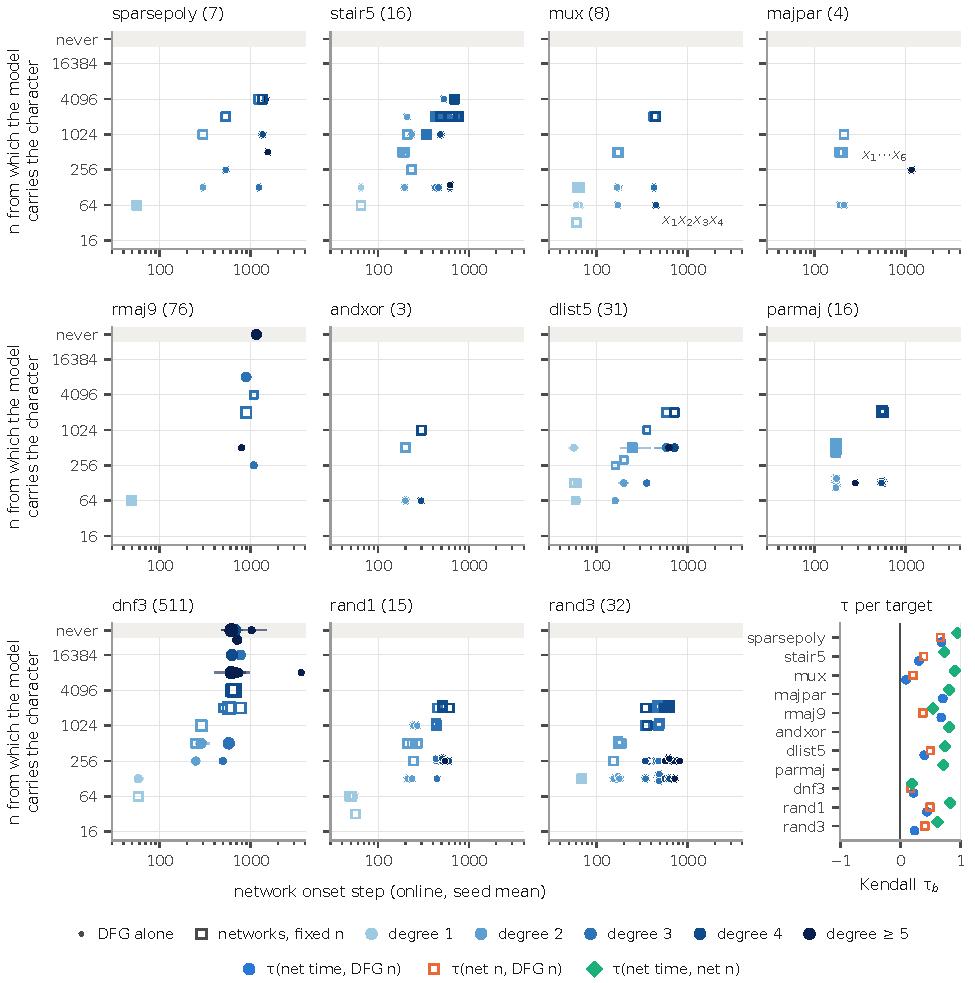
\includegraphics[width=\linewidth]{figures/fig_dyn_order.pdf}
\caption{The order of acquisition, DFG alone against the Part~5 networks \status{Numerical}. One panel per target, with its number of non-constant Fourier characters on the relevant inputs; each point is a character. $x$: the networks' onset step online (the seed-mean learned fraction reaches $1/2$ for good, log-interpolated). $y$: the smallest grid size from which the final model carries the character (learned fraction $\ge1/2$, and $\ge0.4$ at every larger $n$). Filled: DFG alone's least-squares function, median of 3 seeds. Open: the networks of the fixed-$n$ study, median of 3 seeds, $|S|\le4$ only. Grey band: never within $n\le16384$. Colour: degree. For rmaj9, dlist5 and dnf3 there is one marker per (degree, $|\hat f(S)|$) group, at the group's median, with area $\propto\sqrt{\text{count}}$ and a bar over the 10--90\% range of the network onsets. Coinciding points are offset vertically by up to $\pm0.26$ doublings. dnf3's open squares for $|\hat f(S)|\le0.027$ are dominated by the noise of the networks' estimate. Last panel: the three Kendall $\tau_b$ of \cref{tab:dyn-order}b per target; ties leave andxor and parmaj without a $\tau$ against DFG's $n$ order, and majpar without the like-for-like one. Re-plotted from \repo{study/part11/interp/order/tables/order_chars.csv} and \texttt{order\_numbers.json}; the analysis' own figure is \repo{study/part11/interp/order/figures/fig_order.pdf}.}
\label{fig:dyn-order}
\end{figure}
